\begin{figure}[H]
\centering
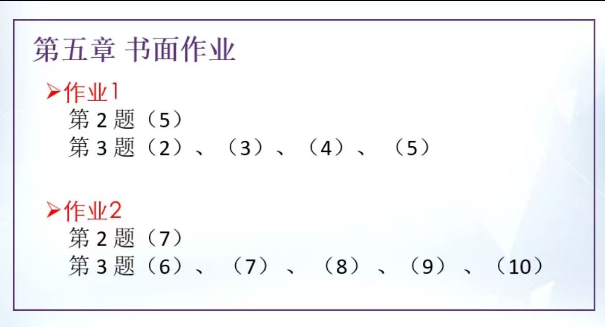
\includegraphics[width=\textwidth]{hw5-2025051319.png}
% \caption{}
\label{}
\end{figure}

\begin{figure}[H]
\centering
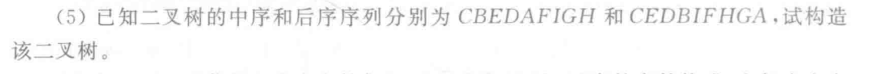
\includegraphics[width=\textwidth]{1-hw5-2025051319.png}
% \caption{}
\label{}
\end{figure}

\begin{figure}[H]
\centering
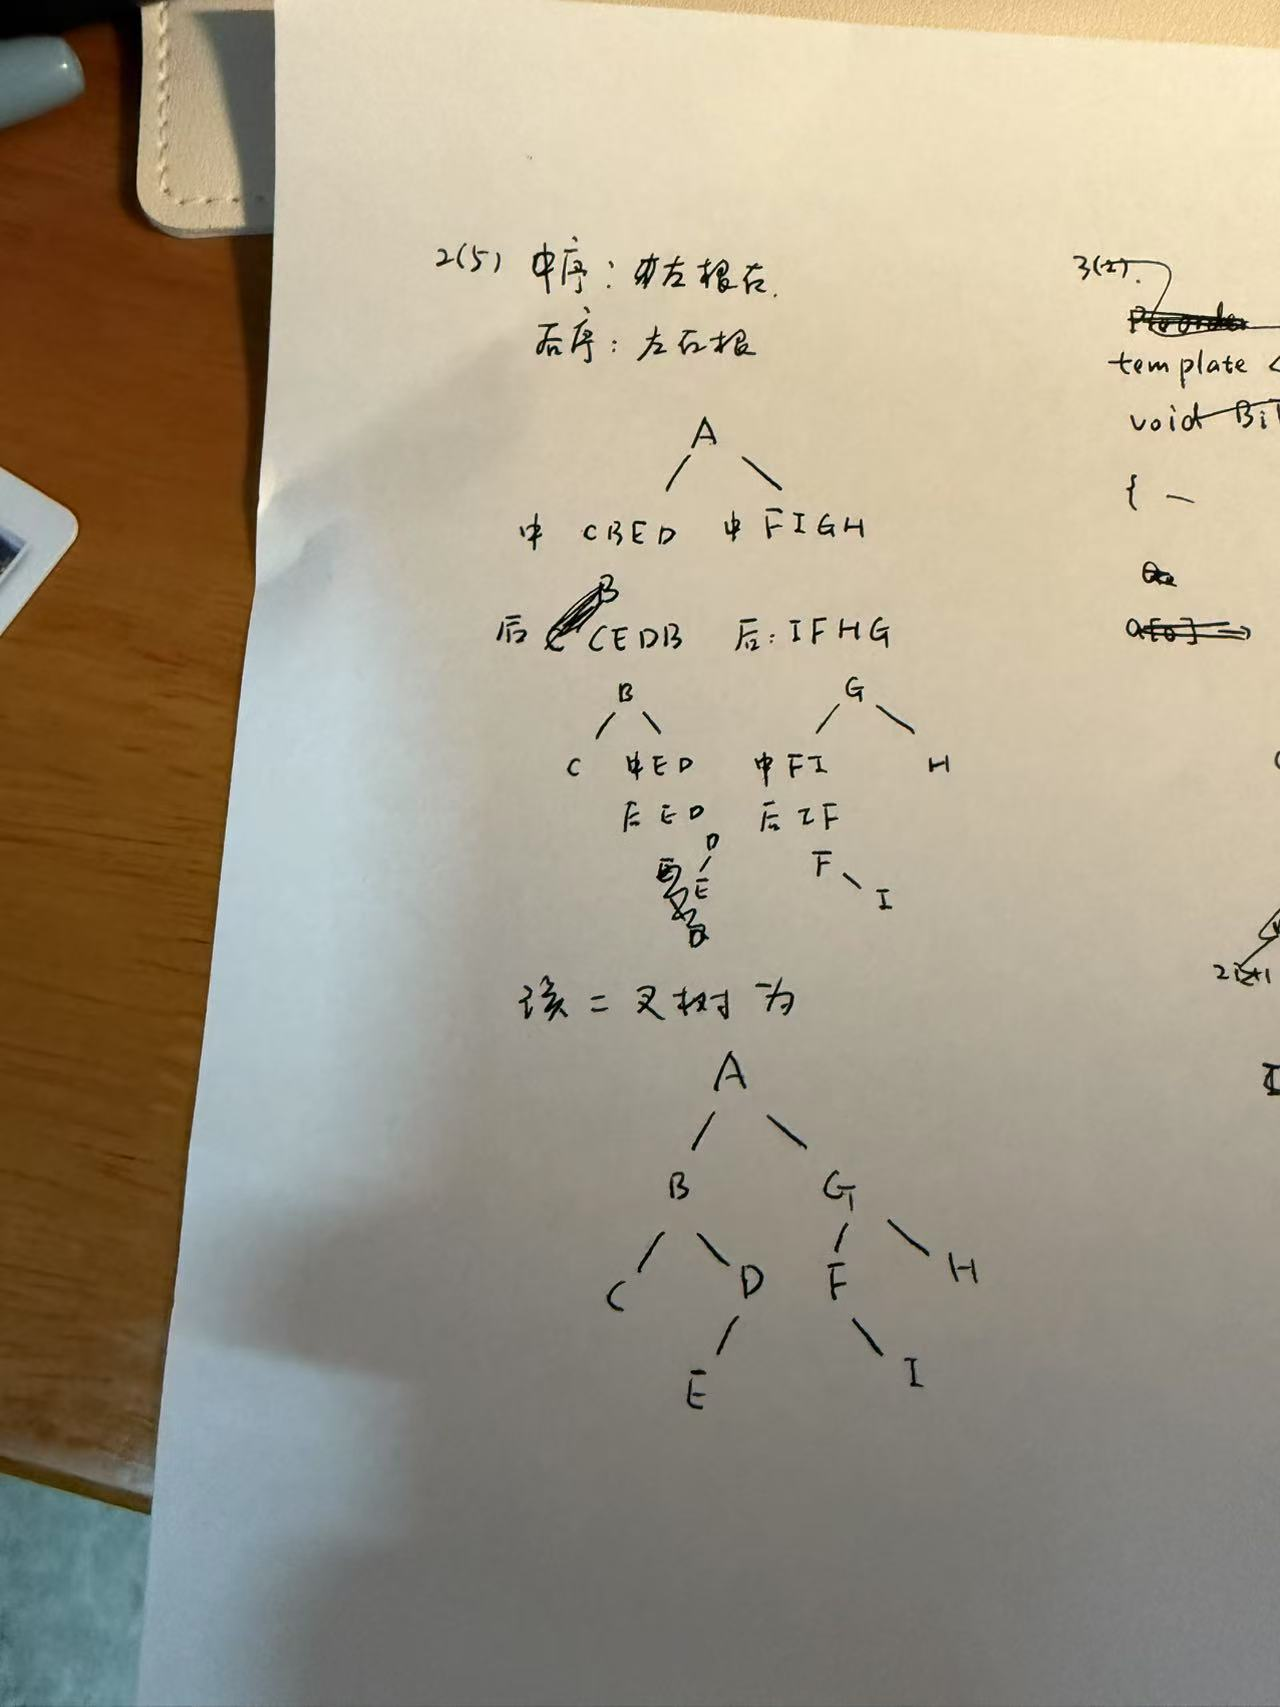
\includegraphics[width=\textwidth]{acffb707e7de42674f96ce8cf7a8031f.jpg}
% \caption{}
\label{}
\end{figure}
\begin{figure}[H]
\centering
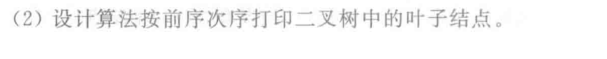
\includegraphics[width=\textwidth]{2-hw5-2025051319.png}
% \caption{}
\label{}
\end{figure}

\textbf{二叉树的叶子}是指二叉树中没有子节点的节点。 它们的度数为零。

\begin{lstlisting}[language=C++]
template<typename DataType>
void BiTree<DataType>:: PrintLeaf(BiNode<DataType> *bt)
{
    if (bt == NULL) return;
    else{
        if (bt->lchild == NULL && bt->rchild == NULL) 
            cout << bt->data << "\t";
        else{
            PrintLeaf(bt->lchild);
            PrintLeaf(bt->rchild);
        }
    }
}
\end{lstlisting}
\begin{figure}[H]
\centering
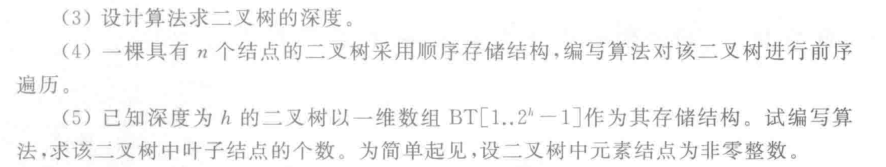
\includegraphics[width=\textwidth]{3-hw5-2025051319.png}
% \caption{}
\label{}
\end{figure}

\begin{lstlisting}[language=C++]
template<typename DataType>
int Depth(BiNode<DataType> *bt) {
    if (bt == NULL) {
        return 0; // 空树0个节点
    }
    int leftDepth = Depth(bt->lchild);
    int rightDepth = Depth(bt->rchild);
    return 1 + std::max(leftDepth, rightDepth);
}
\end{lstlisting}
\begin{lstlisting}[language=C++]
// 简要的前序遍历递归函数
// tree: 顺序存储的二叉树 (用vector<optional<T>>表示)
// index: 当前节点的索引
void preorder_sequential_brief(const std::vector<std::optional<int>>& tree, int index) {
    // 1. 越界或当前节点为空,则返回
    if (index >= tree.size() || !tree[index].has_value()) {
        return;
    }

    // 2. 访问根节点(当前节点)
    std::cout << tree[index].value() << " ";

    // 3. 递归遍历左子树
    preorder_sequential_brief(tree, 2 * index + 1);

    // 4. 递归遍历右子树
    preorder_sequential_brief(tree, 2 * index + 2);
}

\end{lstlisting}
\begin{lstlisting}[language=C++]
int countLeavesCorrected(const std::vector<std::optional<int>>& tree) {
    int leaves = 0;
    if (tree.empty()) {
        return 0;
    }

    for (int i = 0; i < tree.size(); ++i) {
        // Controlla se il nodo corrente esiste
        if (tree[i].has_value()) {
            // Indici dei figli per un genitore basato su 0
            int left_child_idx = 2 * i + 1;
            int right_child_idx = 2 * i + 2;

            bool has_left_child = false;
            if (left_child_idx < tree.size() && tree[left_child_idx].has_value()) {
                has_left_child = true;
            }

            bool has_right_child = false;
            if (right_child_idx < tree.size() && tree[right_child_idx].has_value()) {
                has_right_child = true;
            }

            // Se non ha figli (esistenti), è una foglia
            if (!has_left_child && !has_right_child) {
                leaves++;
            }
        }
    }
    return leaves;
}
\end{lstlisting}
\begin{figure}[H]
\centering
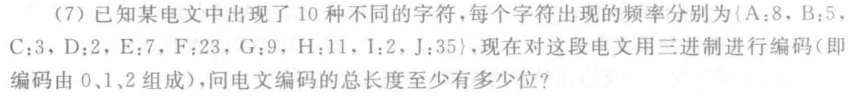
\includegraphics[width=\textwidth]{4-hw5-2025051319.png}
% \caption{}
\label{}
\end{figure}

这是一个典型的霍夫曼编码问题,但是是针对三进制(而不是通常的二进制)进行的。其核心思想是构建一个三叉霍夫曼树。

\textbf{步骤1:准备数据和处理三进制的特殊情况}

给定字符及其频率:

A: 8

B: 5

C: 3

D: 2

E: 7

F: 23

G: 9

H: 11

I: 2

J: 35

共有 n = 10 种不同的字符。

对于k进制霍夫曼编码,有一个要求是 (n - 1) \% (k - 1) 必须等于0,这样才能保证每次合并k个节点最后能形成一棵完整的k叉树。

在这里,n = 10,k = 3 (三进制)。

所以,k - 1 = 2。

计算 (n - 1) \% (k - 1) = (10 - 1) \% 2 = 9 \% 2 = 1。

由于结果不为0,我们需要添加额外的“哑”节点(频率为0),直到满足条件。

需要添加的哑节点数量 m = (k - 1) - ((n - 1) \% (k - 1)) (如果余数不为0)。

m = 2 - 1 = 1。

所以,我们需要添加1个频率为0的哑节点。

现在,我们有 n' = n + 1 = 10 + 1 = 11 个节点(包括哑节点)。

新的频率列表(未排序):

\{A:8, B:5, C:3, D:2, E:7, F:23, G:9, H:11, I:2, J:35, Dummy:0\}

\textbf{步骤2:构建三叉霍夫曼树}

按照霍夫曼算法的步骤,每次选取当前频率最小的3个节点合并成一个新的父节点,新节点的频率是这3个子节点频率之和。重复此过程,直到只剩下一个节点(树根)。

\begin{enumerate}
	\item 排序当前所有节点(包括哑节点)的频率:
\{Dummy:0, D:2, I:2, C:3, B:5, E:7, A:8, G:9, H:11, F:23, J:35\}
	\item \textbf{第一次合并:}
	\begin{itemize}
		\item 选取最小的3个:Dummy(0), D(2), I(2)
		\item 合并得到新节点 N1,频率 = 0 + 2 + 2 = 4
		\item 剩余节点及频率:\{C:3, N1:4, B:5, E:7, A:8, G:9, H:11, F:23, J:35\}
		\item 重新排序:\{C:3, N1:4, B:5, E:7, A:8, G:9, H:11, F:23, J:35\}
	\end{itemize}
	\item \textbf{第二次合并:}
	\begin{itemize}
		\item 选取最小的3个:C(3), N1(4), B(5)
		\item 合并得到新节点 N2,频率 = 3 + 4 + 5 = 12
		\item 剩余节点及频率:\{E:7, A:8, G:9, H:11, N2:12, F:23, J:35\}
		\item 重新排序:\{E:7, A:8, G:9, H:11, N2:12, F:23, J:35\}
	\end{itemize}
	\item \textbf{第三次合并:}
	\begin{itemize}
		\item 选取最小的3个:E(7), A(8), G(9)
		\item 合并得到新节点 N3,频率 = 7 + 8 + 9 = 24
		\item 剩余节点及频率:\{H:11, N2:12, F:23, N3:24, J:35\}
		\item 重新排序:\{H:11, N2:12, F:23, N3:24, J:35\}
	\end{itemize}
	\item \textbf{第四次合并:}
	\begin{itemize}
		\item 选取最小的3个:H(11), N2(12), F(23)
		\item 合并得到新节点 N4,频率 = 11 + 12 + 23 = 46
		\item 剩余节点及频率:\{N3:24, J:35, N4:46\}
		\item 重新排序:\{N3:24, J:35, N4:46\}
	\end{itemize}
	\item \textbf{第五次合并(最后一次):}
	\begin{itemize}
		\item 选取最小的3个:N3(24), J(35), N4(46)
		\item 合并得到新节点 N5 (根节点),频率 = 24 + 35 + 46 = 105
		\item (总频率为 8+5+3+2+7+23+9+11+2+35 = 105,与根节点频率一致)
	\end{itemize}
\end{enumerate}

\textbf{步骤3:计算电文编码的总长度}

电文编码的总长度可以通过两种等效的方式计算:

\begin{enumerate}
	\item \textbf{Σ (字符频率 × 字符编码长度)}:这需要我们实际构造出编码。
	\item \textbf{所有非叶子节点(内部节点,包括根节点)的频率之和}:这是霍夫曼编码的一个重要性质,对于k进制霍夫曼编码同样适用。这种方法更简单,因为它不需要实际分配编码。
\end{enumerate}

我们使用第二种方法。内部节点是我们在合并过程中创建的节点:N1, N2, N3, N4, N5。

它们的频率分别是:

\begin{itemize}
	\item N1: 4
	\item N2: 12
	\item N3: 24
	\item N4: 46
	\item N5: 105
\end{itemize}

电文编码的总长度至少为 = 4 + 12 + 24 + 46 + 105 = \textbf{191} 位。

验证(可选,通过计算每个字符的编码长度):

从构建的树反向追溯,可以得到每个叶子节点的深度,即其编码长度:

\begin{itemize}
	\item N5 (根)
	\begin{itemize}
		\item N3 (深度1)
		\begin{itemize}
			\item E (深度2)
			\item A (深度2)
			\item G (深度2)
		\end{itemize}
		\item J (深度1)
		\item N4 (深度1)
		\begin{itemize}
			\item H (深度2)
			\item N2 (深度2)
			\begin{itemize}
				\item C (深度3)
				\item N1 (深度3)
				\begin{itemize}
					\item Dummy (深度4)
					\item D (深度4)
					\item I (深度4)
				\end{itemize}
				\item B (深度3)
			\end{itemize}
			\item F (深度2)
		\end{itemize}
	\end{itemize}
\end{itemize}

字符编码长度 (l\_i) 和 f\_i * l\_i:

\begin{itemize}
	\item J: 深度1, 频率35 => 35 * 1 = 35
	\item E: 深度2, 频率7 => 7 * 2 = 14
	\item A: 深度2, 频率8 => 8 * 2 = 16
	\item G: 深度2, 频率9 => 9 * 2 = 18
	\item H: 深度2, 频率11 => 11 * 2 = 22
	\item F: 深度2, 频率23 => 23 * 2 = 46
	\item C: 深度3, 频率3 => 3 * 3 = 9
	\item B: 深度3, 频率5 => 5 * 3 = 15
	\item D: 深度4, 频率2 => 2 * 4 = 8
	\item I: 深度4, 频率2 => 2 * 4 = 8
	\item Dummy: 深度4, 频率0 => 0 * 4 = 0
\end{itemize}

总长度 = 35+14+16+18+22+46+9+15+8+8+0 = 191。

两种计算方法结果一致。

结论:

电文编码的总长度至少有 191 位。

\begin{figure}[H]
\centering
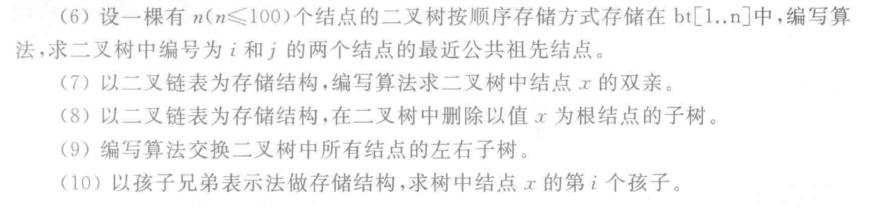
\includegraphics[width=\textwidth]{5-hw5-2025051319.png}
% \caption{}
\label{}
\end{figure}

(6)
顺序存储,$i$ 结点的左孩子为 $2i$ 结点,右孩子为 $2i+1$ 结点. 对于给定的孩子 $i$ ,它的父结点为 $\left\lfloor  \frac{i}{2}  \right\rfloor$. 于是我们只需要不断考虑
\[
\left\lfloor  \frac{i}{2}  \right\rfloor ,\left\lfloor  \frac{\left\lfloor  \frac{i}{2}  \right\rfloor}{2}   \right\rfloor ,\dots
\]
\[
\left\lfloor  \frac{j}{2}  \right\rfloor ,\left\lfloor  \frac{\left\lfloor  \frac{j}{2}  \right\rfloor}{2}   \right\rfloor ,\dots
\]
直到上面两个数列分别出现最大的相等的项.

\begin{lstlisting}[language=C++]
int findLCA_Simple(int id1, int id2) {
    while (id1 != id2) {
        if (id1 > id2) {
            id1 /= 2;
        } else {
            id2 /= 2;
        }
    }
    return id1;
}
\end{lstlisting}
(7)
遍历二叉链表,若 \lstinline{bt->data == x},则停止遍历,输出 \lstinline{bt}.

\begin{lstlisting}[language=C++]
using NodeValue = int; // Or any other appropriate data type

struct TreeNode {
    NodeValue data;
    TreeNode* leftChild;
    TreeNode* rightChild;
};

TreeNode* findParent_Linked(TreeNode* root, NodeValue x_value) {
    if (root == nullptr || root->data == x_value) {
        return nullptr;
    }

    std::queue<TreeNode*> q;
    q.push(root);

    while (!q.empty()) {
        TreeNode* current_node = q.front();
        q.pop();

        if (current_node->leftChild != nullptr) {
            if (current_node->leftChild->data == x_value) {
                return current_node;
            }
            q.push(current_node->leftChild);
        }

        if (current_node->rightChild != nullptr) {
            if (current_node->rightChild->data == x_value) {
                return current_node;
            }
            q.push(current_node->rightChild);
        }
    }

    return nullptr;
}
\end{lstlisting}
(8)
在 (7) 的基础上,将指向 \lstinline{x} 的指针赋值为 \lstinline{NULL}

\begin{lstlisting}[language=C++]
TreeNode* findParent_Linked(TreeNode* root, NodeValue x_value)
TreeNode* DeleteTree(TreeNode* root, NodeValue x_value){
    p = findParent_Linked(root, x_value);
    p = NULL;
}
\end{lstlisting}
(9)

\begin{lstlisting}[language=C++]
// (9) Swap Left and Right Children of All Nodes
void swapAllChildren_Recursive(TreeNode* node) {
    if (node == nullptr) {
        return;
    }

    // Recursively swap children of subtrees first (post-order action)
    swapAllChildren_Recursive(node->leftChild);
    swapAllChildren_Recursive(node->rightChild);

    // Swap the current node's children
    TreeNode* temp = node->leftChild;
    node->leftChild = node->rightChild;
    node->rightChild = temp;
}
\end{lstlisting}
(10)

\begin{lstlisting}[language=C++]
struct CSNode { // Child-Sibling Node
    NodeValue data;
    CSNode* firstChild;
    CSNode* nextSibling;
};

CSNode* get_ith_Child_CS(CSNode* parentNode, int i) { // i is 1-based
    if (parentNode == nullptr || i <= 0) {
        return nullptr;
    }

    CSNode* currentChild = parentNode->firstChild;
    int count = 1;

    while (currentChild != nullptr && count < i) {
        currentChild = currentChild->nextSibling;
        count++;
    }

    if (count == i) {
        return currentChild;
    }
    return nullptr;
}
\end{lstlisting}